

% This document was generated by the publish-function
% from GNU Octave 4.4.1



\documentclass[10pt]{article}
\usepackage{listings}
\usepackage{mathtools}
\usepackage{amssymb}
\usepackage{graphicx}
\usepackage{hyperref}
\usepackage{xcolor}
\usepackage{titlesec}
\usepackage[utf8]{inputenc}
\usepackage[T1]{fontenc}
\usepackage{lmodern}


\lstset{
language=Octave,
numbers=none,
frame=single,
tabsize=2,
showstringspaces=false,
breaklines=true}


\titleformat*{\section}{\Huge\bfseries}
\titleformat*{\subsection}{\large\bfseries}
\renewcommand{\contentsname}{\Large\bfseries Contents}
\setlength{\parindent}{0pt}

\begin{document}

{\Huge\section*{Homework 1}}

\tableofcontents
\vspace*{4em}



\phantomsection
\addcontentsline{toc}{section}{Part (1)}
\subsection*{Part (1)}

\begin{lstlisting}
myexp(1)
\end{lstlisting}
\begin{lstlisting}[language={},xleftmargin=5pt,frame=none]
ans =  2.7183

\end{lstlisting}
\begin{figure}[!ht]
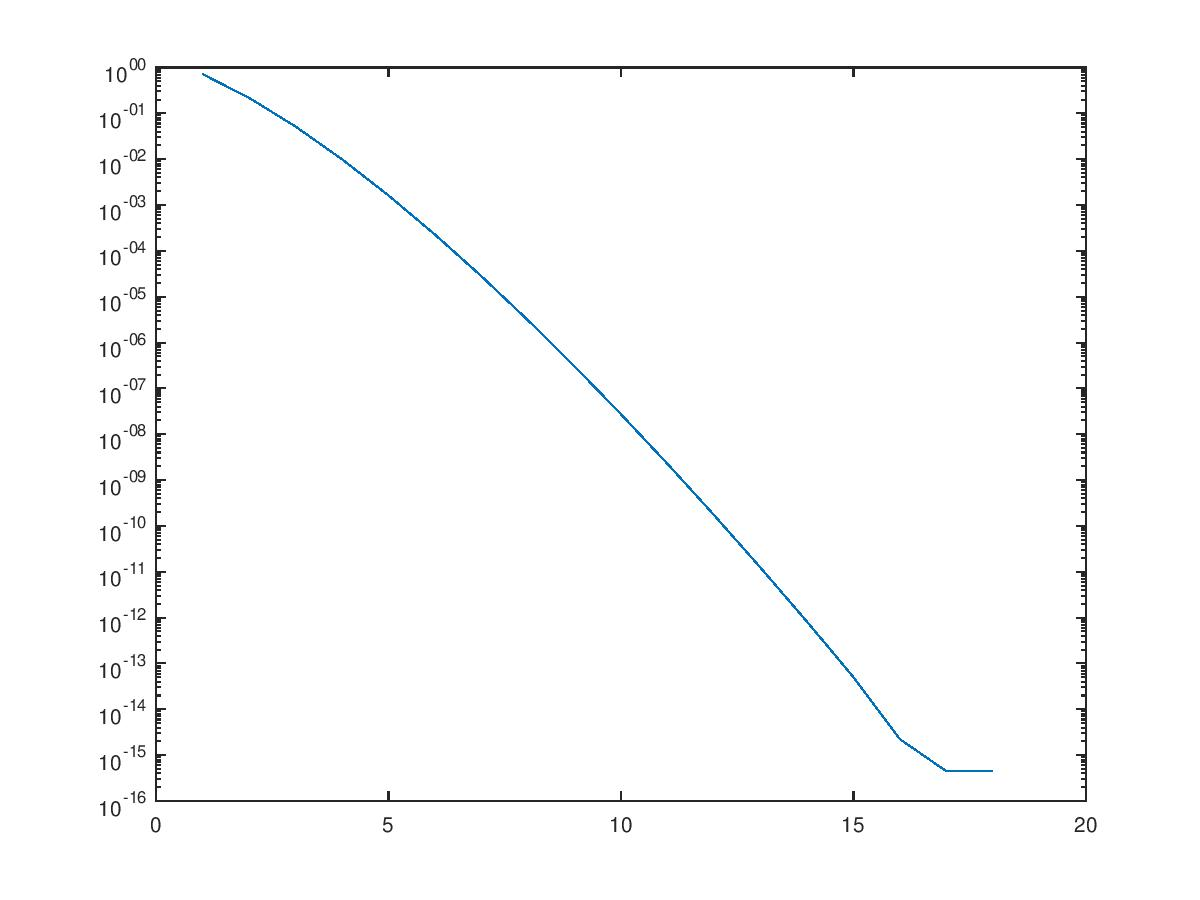
\includegraphics[width=\textwidth]{myscript-1.jpg}
\end{figure}


\phantomsection
\addcontentsline{toc}{section}{Part (2)}
\subsection*{Part (2)}



test $$sin(x) = 1$$

\begin{lstlisting}
myexp(2)
\end{lstlisting}
\begin{lstlisting}[language={},xleftmargin=5pt,frame=none]
ans =  7.3891

\end{lstlisting}
\begin{figure}[!ht]
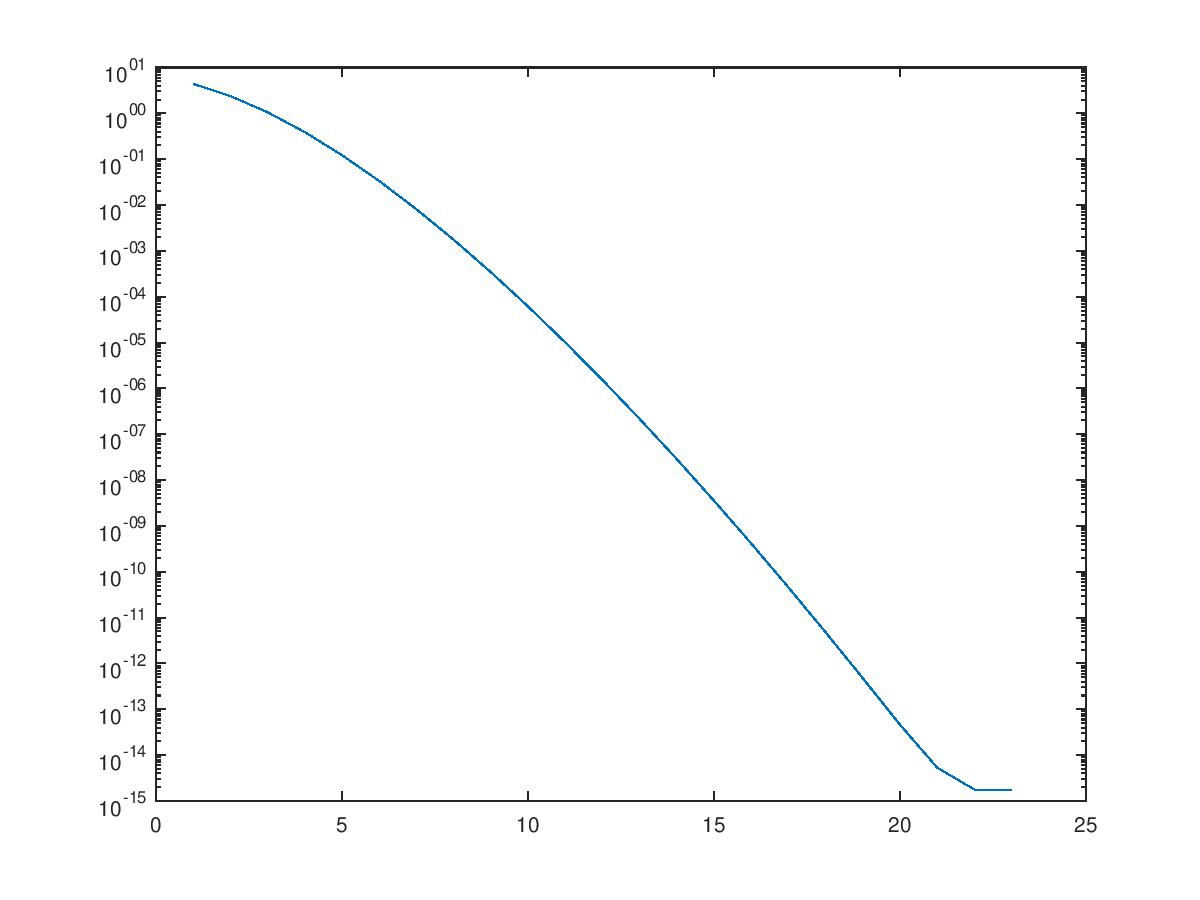
\includegraphics[width=\textwidth]{myscript-2.jpg}
\end{figure}


\end{document}
